\chapter{Indexing for Incremental Proof Development}\label{chapter:indexing-reimplementation}

This chapter presents implementation concerns with supporting incremental program development in \Beluga and \Harpoon.
Some technical debt in those systems is highlighted to justify the reimplementation of the indexing phase.
A formalism and an implementation of identifier resolution for \Beluga are presented to showcase how to efficiently and correctly compute de Bruijn indices in an environment featuring multiple indexing contexts.

\section{Introduction}

% What are aspects of state management that are required to support incremental proof development?
% In what way are state management and exception handling closely linked with respect to interactive proof sessions?

Incremental program development is a broad and open problem in the implementation of interpreters and compilers.
The main challenge with implementing such systems is state invalidation, where editing part of a program causes changes elsewhere, both in the code the user wrote and in the state of the interpreter analysing it.
While reprocessing the affected parts of the code from scratch is a valid solution to guarantee soundness, this does not scale efficiently to large programs.
Structured editing obviates some of the issues with state invalidation and the propagation of changes in incremental development.
Indeed, edit actions are scoped to a model of the program as opposed to the program's textual representation itself, which means they have a limited and controlled effect on the structured editor's state.
Mechanisms can then be designed for the interpreter's state to improve its runtime performance in soundly responding to edit actions.

% How do other systems supporting interactive proof sessions handle state management?

Proof assistants providing interactivity through \acp{REPL} and tools for text editors each approach the problem of incremental development in unique ways tailored to their systems.
For instance, constraint-based type systems require mechanisms to keep track of the effects of solving said constraints so that those effects can be undone in the event that type-checking fails for a given program.
Likewise, context-switching between different parts of a program under edit requires updating the state to correctly reflect what identifiers are in scope, both for providing code completion hints and for performing identifier resolution in new terms.
Furthermore, command histories may be implemented to support undoing and redoing edit actions, which should be a necessary feature for proof assistants since users may apply tactics that do not lead to a solution for a given subgoal.
Additionally, incomplete subgoals may be arranged internally as a tree following the structure of a proof to allow navigating between holes.
The successful implementation of these structured editing features hinges on careful management of recorded state to ensure soundness.

The \Abella\footnote{\Abella version \texttt{2.0.8}}~\cite{baelde2014abella} interactive theorem prover has limited support for structurally editing proofs.
Indeed, it leverages a single global state comprised of mutable references with a snapshot mechanism to copy the entire state on every undoable command.
This state notably includes the signature of declarations, the subordination relation on type families, and the list of subgoals that have yet to be proven in the current lemma under edit.
Hence in its interactive mode, \Abella users are restricted to adding new declarations at the end of the session's state.
Indeed, constructing visiting states to other parts of the signature under edit would require rerunning the processing pipeline from scratch.

\Isabelle/\Isar\footnote{\Isabelle2023} implements a system of transitions between immutable state structures to support pure edit actions~\cite{wenzel2023isabelleimpl, wenzel2023isabelleisarref, wenzel2023isabellesys}.
Indeed, most of that system's state, internally referred to as contexts~\cite{ballarin2006interpretation}, is implemented using immutable 2-3~trees to tabulate data, with each context holding a list of all its predecessor states.
The definitions, proofs and terms in the buffer under edit are stored in such contexts.
Undo operations and modification to the signature then proceed by rolling back the contexts to before the edit was done using their lists of predecessors.
Mutable references are leveraged to represent the global state of the kernel, though their usage is limited.
This mutable data is split between synchronized and unsynchronized management strategies, the former adding mutual exclusion locks to references that hold mutable data to enable safe concurrent computations.
Overall, the extensive use of immutable data structures, coupled with synchronization for mutable data, results in degraded memory usage and runtime performance.
Nonetheless, this system allows finer edit actions and ensures that cache invalidations are resolved consistently.

\Agda\footnote{\Agda \texttt{v2.6.4}}~\cite{clffolp, norell2007towards, agda2023} supports incremental interactions with its \Agda mode and its implementation of the language server protocol.
Issuing an edit command with those systems directly affects the text editor's buffer, which provides a seamless editing experience.
Under the hood, this is supported by \Agda's type checking monad, which is an instance of the state monad whose state structure contains most of the mutable and immutable data used throughout the system.
This state includes global configuration parameters, scope information, user-defined notations for parsing, typing contexts for variables as association lists, etc.
It is an agglomeration of all the data used in \Agda's processing pipeline, readily available as a function parameter as opposed to being represented using a global mutable data structure.
This wholly captures the idea of a visiting state over declarations in an \Agda signature.
The main issues when dealing with this type checking monad are performance overheads, and ensuring that state mutations are sound.
To mitigate soundness issues, some interaction kinds have defined scopes to restrict their effect on the type checking state.
In case of bugs arising during edit sessions, separate commands are available to the user to restore the state to earlier checkpoints or to entirely reload the current editor buffer.

\Coq\footnote{\Coq \texttt{v8.18.0}} and the \CoqIDE~\cite{Coq, bertot2013interactive} implement a state transaction machine to efficiently keep track of changes to proofs and their effects on the system's state.
This is backed by a version control system whose design is inspired by \textsc{Git}.
Internally, a \ac{DAG} is created and maintained to represent states as nodes and transactions (or differences) as edges.
Committed changes to the state create branches in the version control system which can then be merged, deleted or checked out.
The actual data to use at a given state in this system is reconstructed by traversing the \ac{DAG} from the root node to the target node while applying the effects encoded in each visited edge.
Concretely, this version control system is used in \Coq's interactive environment when processing vernacular commands, including querying documents, starting proofs, stepping in a proof, and solving a subgoal.

% What are the features desired for Harpoon and Beluga?
% Why do those features help in incremental proof development?

As an interactive frontend for \Beluga, the \Harpoon system is designed such that editing a proof script by way of administrative commands or tactics is guaranteed to preserve the soundness of the proof with respect to the rest of the \Beluga signature.
This includes, among other things, ensuring that input terms are well-typed, that cases analyses cover all possible branches with respect to type family definitions, and that identifiers can be properly resolved once proof scripts are translated into programs.
Chiefly, \Harpoon's administrative commands must work as intended in any valid order of execution so as to ensure that user's work does not get lost.
Just like \Abella, \Isabelle/\Isar, \Coq and \Agda, undoable commands in \Harpoon must undo those commands' effects on both the proof script and the editing state.
Unlike \Abella though, undone commands can be redone, which allows users to move effortlessly forward and backward in the edit history.
One feature that is unique to \Harpoon is the ability to efficiently checkout the proof state for incomplete theorems occurring anywhere in a \Beluga signature.
This enables the development of proofs in a top-down fashion by first stating theorems and lemmas and then proving them, fully or partially, in any order that seems most productive.
This is stronger than \Abella's and \Coq's subgoal deferring feature, which \Harpoon also supports, in that theorems may be declared with respect to different subsets of the signature in the same proof session.

Unfortunately, case studies revealed that the implementation of \Harpoon's theorem-switching feature can lead to invalid \Beluga signatures when proof scripts developed out of order are translated into programs.
Indeed, upon checking out an incomplete proof script, the signature is not be reverted back to the state at which that proof is declared.
This effectively means that definitions occurring later in a proof session appear in scope during interactive proof sessions.
To soundly support switching between theorems, the \Beluga system requires a mechanism to rollback the referencing state to the point where theorems are declared.
This prompted the reimplementation of name resolution in \Beluga and \Harpoon to support visiting states.

\section{The Legacy Indexing Phase}

% What is indexing, more precisely?

As outlined in section~\ref{section:beluga-implementation}, the indexing phase of \Beluga's processing pipeline is responsible for converting external syntax trees to corresponding approximate syntax trees.
Specifically, references to constants are replaced with their corresponding symbolic identifiers defined in the signature reconstruction store, and variables are replaced with their corresponding de Bruijn indices.
This allows for later phases of semantic analysis (such as type-checking and termination analysis) to efficiently look up constant definitions and resolve variables to their binders without having to keep track of the identifiers in scope.
In the implementation, not all variables are replaced with de Bruijn indices during indexing because binders for implicit parameters are not present in the \ac{AST}; these are introduced during the abstraction phase~\cite{germain2010implementation}.

% What features are required of indexing?

% What was the legacy implementation of indexing? Why did it require reimplementation?

The legacy implementation of indexing is additionally responsible for disambiguating the application of user-defined operators since that phase keeps track of constants as they are introduced in the signature.
This disambiguation leverages Dijkstra's shunting-yard algorithm as opposed to the recursive descent parsing algorithm presented in section~\ref{section:parsing-user-defined-operators}.
In the revised system, this responsibility has been moved to its own disambiguation phase, as presented in section~\ref{section:lexing-parsing-disambiguation}, which requires its own implementation of name resolution.
While this refactoring could have been sufficient in simplifying the processing pipeline, it uncovered significant technical debt and issues having to do with the way identifiers are handled during indexing.

The overarching store illustrated in figure~\ref{figure:legacy-beluga-processing-pipeline} records the constant declarations encountered during signature reconstruction.
These declarations are arranged in tables, with one table per kind of constant declaration, as illustrated in figure~\ref{figure:referencing-environment-architecture}.
Variable declarations, on the other hand, are arranged separately in association lists.
This guarantees that there is no overlap between identifiers referring to objects of different kinds since they are not looked up in the same table or association list, which effectively creates distinct namespaces for them.
For instance, \LF type-level and term-level constants have their own declaration tables, separate from computation-level type constants and constructors.
This design aims at ensuring that variables and constants originating from the \LF, meta or computation levels do not end up appearing in terms of a different level~\cite{germain2010implementation}.
Unfortunately, without having a unique table representing an entire referencing environment, name resolution in the presence of shadowing proves obtuse and leads to unexpected results when coupled with overloading of identifiers.
Indeed, when a constant identifier is resolved during indexing, the declaration tables in the store are looked up in a pre-defined order.
As such, identifier lookups to not respect the global insertion order of constant and variable declarations.
Instead, they are looked up first with respect to the order of identifier kinds, and then by the declaration order within the table for that identifier kind.
Consequently, parts of the referencing environment do not exist depending on the expected kind of variable or constant encountered in the \ac{AST}.
For example, it is impossible in \Beluga~\texttt{v1.0} for computation-level coinductive type constant to shadow an inductive one simply because the declaration table for the former kind is always looked up after the declaration table for the latter kind.
Likewise, since identifiers at the meta-level and at the computation-level are kept separate, invalid references to computation-level objects in boxed terms are undetectable as they are instead systematically interpreted as free meta-variables.
Counterintuitively, different parts of the referencing environment can also be interleaved in one program with this split table and association lists approach.
Indeed, one can introduce a binder for a meta-level variable and another for a computation-level variable, both using the same identifier, and be able to use both meanings for that identifier in meta-level and computation-level expressions respectively because they effectively occupy different namespaces.
The contrived but valid example program \verb*|f| below illustrates this: the colour-coded identifiers ${\color{red}{g}}$ and ${\color{magenta}{x}}$ are in $\Delta$, and ${\color{blue}{g}}$ and ${\color{teal}{x}}$ are in $\Gamma$, in such a way that the function's body uses both overloaded meanings of those identifiers.
This is admissible because only one namespace is made available at a time based on the variant of \ac{AST} node the identifier lies in.
\bigskip
\begin{Verbatim}[commandchars=\\\{\}, baselinestretch=1]
{\verbbf{LF}} tm : {\verbbf{type}} = ...;
{\verbbf{schema}} ctx = ...;
{\verbbf{inductive}} Ex : {\verbbf{ctype}} = ...;

{\verbbf{rec}} f : {\{g : ctx\}} -> [g |- tm] -> Ex -> Ex =
  {\verbbf{mlam}} {\color{red}{g}} => {\verbbf{fn}} {\color{blue}{g}} => {\verbbf{fn}} {\color{teal}{x}} => {\verbbf{let}} [_ |- {\color{magenta}{x}}] = {\color{blue}{g}} {\verbbf{in}} f [{\color{red}{g}}] [{\color{red}{g}} |- {\color{magenta}{x}}] {\color{teal}{x}};
\end{Verbatim}
This overloading does not translate well in proofs on paper since that results in an identifier being used to refer to two distinct objects in the same proof.
It also challenges the identifier scoping rules suggested by \Beluga's concrete syntax.
An error message like the following one should be raised instead to ensure proper lexical scoping of variable declarations.
\bigskip
\begin{Verbatim}[commandchars=\\\{\}, baselinestretch=1]
\verbpbf{File "example.bel", line 6, column 52:}  
6 |  mlam g => fn g => fn x => let [_ |- x] = g in f [g] [g |- x] x;
                                                      \verbrbf{^}             
\verbrbf{Error:} Expected a context variable.
    \verbpbf{File "example.bel", line 6, column 16:}
    6 |  mlam g => fn g => fn x => let [_ |- x] = g in f [g] [g |- x] x;
                      \verbrbf{^}                                                 
    \verbrbf{Error:} g is a bound computation variable.
\end{Verbatim}

\begin{figure}[htb]
\centering
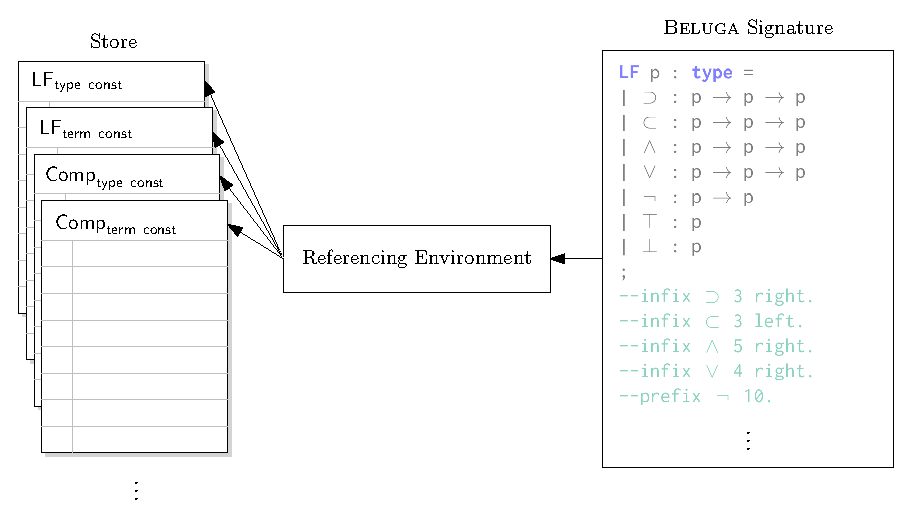
\includegraphics{figures/referencing-environment-architecture.eps}
\caption[Role of the referencing environment in \Beluga]{%
Diagram of the referencing environment structure as a mediator between the \Beluga signature and the reconstruction store for name resolution.
}
\label{figure:referencing-environment-architecture}
\end{figure}

Additionally, the legacy indexing algorithm is tightly coupled and implicitly dependent on the store of constants depicted in figure~\ref{figure:legacy-beluga-processing-pipeline}.
This means that external mutations to that store affect the output of functions responsible for identifier resolution.
As outlined in section~\ref{section:intro-state-management}, this design is only suitable for a single pass through the processing pipeline since only then is the store's state is consistent with how the \ac{AST} is traversed.
Indexing is only explicitly parameterized with respect to association lists for variable declarations.
This allows \Harpoon and \ac{REPL} sessions instantiated in the very last program declared in a \Beluga signature to stay consistent with identifier resolution during signature reconstruction.
Indeed, when navigating to a different \Harpoon subgoal, the variable bindings introduced by the current subgoal can be discarded and replaced with those of the new subgoal.
Incremental proof development sessions initiated on holes located anywhere else but the last declaration in the signature may result in invalid programs being generated.
Since the store of constants is stuck at the state it ends up in after the signature is reconstructed, checking out those holes incorrectly brings later constants in scope.
This can lead to shadowing of constants required for the proof development.
In order to ensure soundness of incremental proof development with holes in proof scripts located anywhere in a signature, it is necessary for indexing to be explicitly parameterized over the entire referencing environment as opposed to just the stores for variables.

% TODO: Add example?

The aforementioned incongruities in name resolution and tight coupling with the signature reconstruction store motivate the reimplementation of the indexing phase to use one uniform namespace while ensuring that identifiers from different domains cannot occur in terms in which they don't belong.
Without having types available at this stage of processing, the accidental feature of identifier overloading had to be discarded to avoid postponing ambiguous references to type-checking.

\section{Uniform Indexing}\label{section:indexing}

% What is uniform indexing?

Uniform indexing is the conversion from a named \ac{AST} to a locally nameless \ac{AST} in a single pass and using a single lookup structure for all identifier kinds.
By parameterizing procedures dealing with named binders to use such a lookup structure, we can resolve the soundness issue with holes in programs by explicitly managing the state of that structure to correctly reflect what identifiers are in scope.
For \Beluga, implementing this requires having a merged view of the declaration tables for constants and variables so as to uniformly know what identifiers are in scope at any given \ac{AST} node.
In particular, variable identifiers in the \LF context, the meta-level context, and the computation-level context as illustrated in figure~\ref{figure:indexing-contexts}, which were designed to belong to different identifier worlds~\cite{ferreira2012compiler}, now have to be mixed together for name resolution.
Subsequent passes of the processing pipeline such as type reconstruction and type-checking may still safely treat those contexts as separate entities using the locally nameless \ac{AST}.
To solve the problem of uniform indexing, some definitions are in order.

\begin{figure}[H]
\centering
\begin{tabular}{lcll}
\LF contexts & $\Psi$ & $\Coloneqq$ & $\cdot \mid \Psi, x : A $\\
Meta-level contexts & $\Delta$ & $\Coloneqq$ & $\cdot \mid \Delta, X : U $\\
Computation-level context & $\Gamma$ & $\Coloneqq$ & $\cdot \mid \Gamma, x : \tau$
\end{tabular}
\caption[Indexing contexts in \Beluga]{%
Definition of the indexing contexts in \Beluga, with respect to which variables are indexed as de Bruijn indices.
This builds upon the definitions of figure~\ref{figure:internal-syntax}.
}
\label{figure:indexing-contexts}
\end{figure}

% TODO: State more prominently, not just in the text.
% TODO: But the variables in \Psi, \Delta and \Gamma are still treated separately during type reconstruction, type-checking...

% What are frames?
% What are scopes?
% What are fully qualified identifiers?
% What are referencing environments?

A \textit{frame} is a lexical region of an \ac{AST} wherein variable declarations and references can be made.
A \textit{scope} is a frame in which name resolution is uniform, meaning that references are resolved to the same declaration site irrespective of the \ac{AST} node in the scope.
Whereas declarations can shadow each other within a frame, all declarations have to be distinct in a scope.
%Because of this, shadowing with scopes is only supported by nesting.
A \textit{fully qualified identifier} $x_1.x_2.\cdots.x_n$ is a list of plain identifiers $x_1$, $x_2$, $\dots$, $x_n$ separated by dots denoting projection out of a namespace.
A \textit{referencing environment} in \Beluga is the data structure that holds the associations from fully qualified identifiers to definitions in a signature.
In essence, a referencing environment provides a window over a signature for name resolution, and as such its state is restricted to representing one scope at a time.

%The uniform indexing phase is designed as a single sequential traversal of the external named \ac{AST} to map it to the approximate locally nameless \ac{AST}, using the referencing environment as visitor state.
During indexing, the referencing environment is updated by adding or removing identifiers in scope as \ac{AST} nodes are traversed.
This presents the challenge of cohesively handling namespaces for modules, patterns for computation-level pattern-matching expressions, and the computation of de Bruijn indices across different indexing contexts ($\Psi$, $\Delta$ and $\Gamma$).
%This includes name resolution under lambda-expressions and contexts in contextual \LF patterns, as well as distinguishing between pattern variables and bound identifiers.
All the while, indexing has to feature some backtracking mechanism to support incremental proof development in \Harpoon sessions.
It is also worth noting that in the disambiguation phase, where a similar mapping occurs from the parser \ac{AST} to the external \ac{AST}, the visitor state has to additionally keep track of user-defined notations.
This means that whichever structure is used to model referencing environments has to be extensible.

% What motivates the introduction of frames?

Every identifier declaration is allowed to shadow previous declarations in \Beluga.
The only exception to this rule is that identifiers in mutually recursive declarations have to be unique.
Everywhere else, declarations for constants and variables introduce their own scope.
This means that a scope graph~\cite{nameresolution} representation of name resolution for \Beluga programs is essentially a line graph, which is computationally inefficient for name resolution.
As such, the referencing environment is instead modelled and implemented using frames as a basis.

Concretely, a referencing environment is a stack of frames, as illustrated in figure~\ref{figure:referencing-environment-definition}.
Each frame holds a tree of bindings, wherein each node assigns to an identifier a stack of entries and optionally a subtree.
The stacks of bindings provide a means of recalling what earlier definitions were assigned to identifiers in the current frame as the traversal exits a scope.
Namespaces are handled uniformly since every binding may introduce one in the form of a subtree of bindings.
The type of entry in a referencing environment is extensible, which allows for additional kinds of identifier references to be defined, and for data to be added to support different kinds of algorithms relying on the named \ac{AST}.

For indexing specifically, the entries are annotated with labels for the various kinds of declarations in \Beluga signatures (i.e., $\LFTerm$, $\Ctx$, $\CompTerm$, $\LFTypeConst$, $\LFTermConst$, ...), as well as indexing context sizes $|\Psi|$, $|\Delta|$ and $|\Gamma|$ for variables, and symbolic identifiers $\tilde a$ and $\tilde c$ for constants in the signature reconstruction store.
Indexing context sizes are also kept track of in the structure for bindings to support computing de Bruijn indices.

\begin{figure}[H]
\centering
{\footnotesize
\begin{tabular}{lrcl}
Referencing environment & $\Xi$ & $\Coloneqq$ & $ \cdot \mid \Xi; \mathcal{F} $\\
Frame & $ \mathcal{F} $ & $ \Coloneqq $ & $ \Frame \mid \Module \mid \Pattern $\\
Plain frame & $ \Frame $ & $ \Coloneqq $ & $ \Bindings $\\
Module frame & $ \Module $ & $ \Coloneqq $ & $ (\Bindings, \BindingsTree) $\\
Pattern frame & $ \Pattern $ & $ \Coloneqq $ & $ (\Bindings_{\text{p}}, \Bindings_{\text{e}}) $\\
Bindings & $ \Bindings $ & $ \Coloneqq $ & $ (\BindingsTree, |\Psi|, |\Delta|, |\Gamma|) $\\
Binding tree & $ \BindingsTree $ & $ \Coloneqq $ & $ \set{x_i \mapsto \mathcal{S}_i}_{i \in \set{1, 2, \dots, n}} $\\
Entry stack & $ \mathcal{S} $ & $ \Coloneqq $ & $ \cdot \mid \mathcal{S}; (e, \BindingsTree) $\\
Entry & $ e $ & $ \Coloneqq $ & $ \cdots \mid (\LFTerm, |\Psi|) \mid (\Ctx, |\Delta|) \mid (\CompTerm, |\Gamma|) $\\
&&& $ \phantom{\cdots} \mid (\LFTypeConst, \tilde a) \mid (\LFTermConst, \tilde c) $
\end{tabular}
}
\caption[Definition of referencing environments for \Beluga programs]{%
Definition of referencing environments for \Beluga programs, assigning stacks of entries to identifiers with a stack of frames.
}
\label{figure:referencing-environment-definition}
\end{figure}

The entry stacks and bindings tree structures of figure~\ref{figure:referencing-environment-definition} can be flattened into an association list by keeping track of the insertion order for bindings.
This is used for presentation purposes, with $[x_1 : \tau_1, x_2 : \tau_2, \cdots, x_n : \tau_n]_\Module$ denoting a module frame with bindings $x_1 : \tau_1$, $x_2 : \tau_2$, ..., $x_n : \tau_n$ like in figure~\ref{figure:example-reference-environment-formalism}.
To illustrate which identifiers are introduced in scope by a frame, the set of toplevel identifiers for frames and binding trees is defined in figure~\ref{figure:definition-domain-frames}.
%Then, the right-to-left association list corresponding to a referencing environment $\Xi = \mathcal{F}_1; \mathcal{F}_2; \cdots; \mathcal{F}_n$ is $\Domain(\mathcal{F}_1) \oplus \Domain(\mathcal{F}_2) \oplus \cdots \oplus \Domain(\mathcal{F}_n)$ where $\oplus$ denotes concatenation.

\begin{figure}[H]
\centering
{\footnotesize
\begin{tabular}{lcll}
$\Domain(\Frame)$ & $=$ & $\Domain(\Bindings)$ & when $\Frame = \Bindings$\\
$\Domain(\Module)$ & $=$ & $\Domain(\Bindings)$ & when $\Module = (\Bindings, \_)$\\
$\Domain(\Pattern)$ & $=$ & $\Domain(\Bindings_{\text{p}})$ & when $\Pattern = (\Bindings_{\text{p}}, \_)$\\
$\Domain(\Bindings)$ & $=$ & $\Domain(\BindingsTree)$ & when $\Bindings=(\BindingsTree, \_, \_, \_)$\\
$\Domain(\BindingsTree)$ & $=$ & $\set{x_1, x_2, \dots, x_n}$ & when $\BindingsTree = \set{x_i \mapsto \EntryStack_i}_{i \in \set{1, 2, \dots, n}}$
\end{tabular}
}
\caption[Definition of the domain of frames]{%
Definition of the $\Domain$ of frames in a \Beluga referencing environment.
}
\label{figure:definition-domain-frames}
\end{figure}

\subsection{Frames for Patterns and Modules}

% What kinds of frames will we deal with?

Since \Beluga supports defining constants in modules, and pattern-matching in computation-level programs, three distinct kinds of frames are designed to operate differently in the way bindings are added or looked up.
Figure~\ref{figure:frames-addition-removal-definition} illustrates how these frames are added to and removed from referencing environments to support those features.

\begin{enumerate}
\item
\textit{Plain frames} $\Frame$: this kind of frame does not have additional mechanisms.
Plain frames are suitable for introducing multiple identifiers in such a way that they can be efficiently removed by discarding the frame entirely.
\item
\textit{Module frames} $\Module$: constants added to this kind of frame are either private or public.
Only public constant declarations are exported from the module they appear in when it is opened, in which case they are brought in scope.
This ensures that constants and notations imported from external modules are not reexported when the module is opened elsewhere.
To support this, when a constant binding is added to a module frame $(\Bindings, \BindingsTree)$, it is added to both $\Bindings$ for name resolution, and to the tree of exported constants $\BindingsTree$ for opening modules.
This is illustrated in figure~\ref{figure:referencing-environment-modules}.
\item
\textit{Pattern frames} $\Pattern$: variables added to this kind of frame are inner pattern-bound or pattern variables.
Inner pattern-bound variables are introduced by binders in the pattern, like $c$ and $x$ in the contextual lambda term pattern $[c : \mathsf{tm} \rightarrow \mathsf{tm} \vdash \mathsf{lam} (\backslash x. c\; x)]$.
Pattern variables on the other hand are free variables in the pattern, which become bound variables in the body of the match case.
For a pattern frame $(\Bindings_{\text{p}}, \Bindings_{\text{e}})$, the bindings in $\Bindings_{\text{p}}$ are used for name resolution in the pattern, whereas the bindings in $\Bindings_{\text{e}}$ are only used for name resolution in the body of the pattern-matching branch.
This means that inner pattern-bound variables are added to $\Bindings_{\text{p}}$, and free pattern variables are added to $\Bindings_{\text{e}}$.
Because of the way meta-level abstractions are automatically reconstructed for patterns, free meta-variables are both inner pattern-bound and pattern variables.
This allows duplicate occurrences of free meta-variables to occur in a pattern.
\end{enumerate}

\begin{figure}[H]
\begin{subfigure}{\linewidth}
\begin{Verbatim}[commandchars=\\\{\}, baselinestretch=1, numbers=left]
\verbbf{module} Nat = \verbbf{struct}
  \verbbf{LF} nat : \verbbf{type} =
  | z : nat
  | s : nat \makebox[1em]{→} nat;
  \verbbf{rec} plus : [ \makebox[1em]{⊢} nat] \makebox[1em]{→} [ \makebox[1em]{⊢} nat] \makebox[1em]{→} [ \makebox[1em]{⊢} nat] = \verbhole{?h1};
\verbbf{end}
\verbbf{rec} f : [ \makebox[1em]{⊢} Nat.nat] \makebox[1em]{→} [ \makebox[1em]{⊢} Nat.nat] = \verbhole{?h2};
\verbprag{--open Nat.}
\verbbf{rec} g : [ \makebox[1em]{⊢} nat] \makebox[1em]{→} [ \makebox[1em]{⊢} nat] = \verbhole{?h3};
\end{Verbatim}
\caption[Example \Beluga signature with holes]{%
Excerpt of a \Beluga signature with holes \texttt{\verbhole{?h1}}, \texttt{\verbhole{?h2}} and \texttt{\verbhole{?h3}}.
}
\label{figure:referencing-environment-example}
\end{subfigure}
\par\bigskip
\begin{subfigure}{\linewidth}
\begin{equation*}
\begin{aligned}
\Xi_{\texttt{\verbhole{?h1}}} &= \left[\dots\right]_\Module; \left[\Public{\mathsf{nat}} : \mathsf{LF}_{\mathsf{type\ const}}, \Public{\mathsf{z}} : \mathsf{LF}_{\mathsf{term\ const}}, \Public{\mathsf{s}} : \mathsf{LF}_{\mathsf{term\ const}}, \Public{\mathsf{plus}} : \mathsf{Prog}\right]_\Module\\
\Xi_{\texttt{\verbhole{?h2}}} &= \left[\dots, \Public{\mathsf{Nat}} : \left(\mathsf{Module}, \set{\mathsf{nat} : \_, \mathsf{z} : \_, \mathsf{s} : \_, \mathsf{plus} : \_}\right), \Public{\mathsf{f}} : \mathsf{Prog}\right]_\Module\\
\Xi_{\texttt{\verbhole{?h3}}} &= \left[\dots, \Public{\mathsf{Nat}} : \_, \Public{\mathsf{f}} : \_, \Private{\mathsf{nat}} : \_, \Private{\mathsf{z}} : \_, \Private{\mathsf{s}} : \_, \Private{\mathsf{plus}} : \_, \Public{\mathsf{g}} : \mathsf{Prog}\right]_\Module
\end{aligned}
\end{equation*}
\caption[Example referencing environments in the formalism]{%
The referencing environments $\Xi_{\texttt{\verbhole{?h1}}}$, $\Xi_{\texttt{\verbhole{?h2}}}$ and $\Xi_{\texttt{\verbhole{?h3}}}$ for the holes $\texttt{\verbhole{?h1}}$, $\texttt{\verbhole{?h2}}$ and $\texttt{\verbhole{?h3}}$ in figure~\ref{figure:referencing-environment-example}, denoted using association lists to illustrate the semantics of opening a module as in figure~\ref{figure:frames-addition-removal-definition}.
Some annotations to the bindings are omitted for brevity.
Bindings annotated with an asterisk $*$ denote constants that are exported from the module.
\Beluga does not treat files as modules like in \OCaml, so all declarations in the toplevel module carry over to the next signature file in the project configuration.
Nested modules, however, respect the semantics of exporting declarations.
}
\label{figure:example-reference-environment-formalism}
\end{subfigure}
\caption[Handling of modules in referencing environments]{Handling of modules in referencing environments.}
\label{figure:referencing-environment-modules}
\end{figure}%
\begin{figure}\ContinuedFloat
\begin{subfigure}{\linewidth}
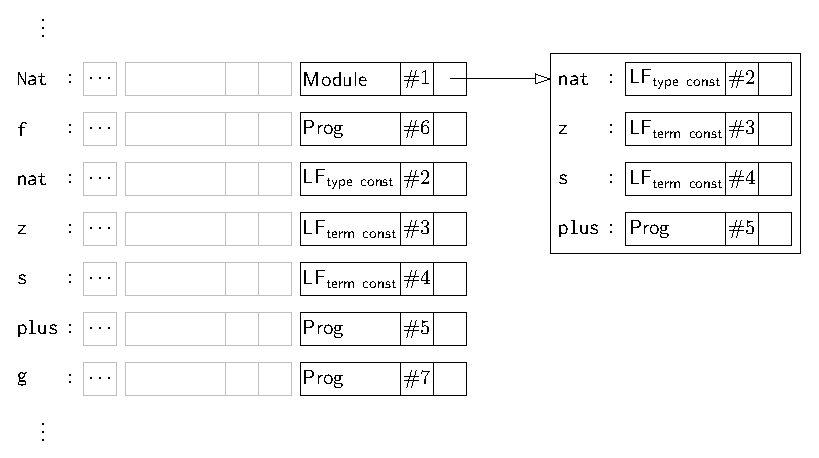
\includegraphics{figures/referencing-environment-implementation.eps}
\caption[]{%
Diagram of the referencing environment at hole \texttt{\verbhole{?h3}} from figure~\ref{figure:referencing-environment-example} as it is implemented in \Beluga~\texttt{v1.1} using dictionaries and stacks.
The identifiers on the left are part of the toplevel module frame, and are each associated with a stack of bindings, with the most recent binding on the right end of the stack.
The numbers \texttt{\#1}, \texttt{\#2}, ..., \texttt{\#7} denote the symbolic identifiers generated during indexing and associated with the constants in the signature reconstruction store.
The aliases introduced by opening module \texttt{Nat} are handled properly, such that constant \texttt{\#3} can be referenced either as \texttt{Nat.z} or \texttt{z} at that point in the signature.
}
\label{figure:referencing-environment-implementation}
\end{subfigure}
\caption[]{Handling of modules in referencing environments (cont.).}
\end{figure}

\begin{figure}[H]
\centering
\makebox[\textwidth][c]{%
{\footnotesize
\begin{tabular}{lcll}
$\operatorname{enter\_frame}(\Xi; \Frame) $ & $=$ & $ \Xi; \Frame; (\{\}, |\Psi|, |\Delta|, |\Gamma|)$ & $\Frame = (\_, |\Psi|, |\Delta|, |\Gamma|)$\\
$\operatorname{enter\_frame}(\Xi; \Module) $ & $=$ & $ \Xi; \Module; (\{\}, |\Psi|, |\Delta|, |\Gamma|)$ & $\Module = ((\_, |\Psi|, |\Delta|, |\Gamma|), \_)$\\
$\operatorname{leave\_frame}(\Xi; \Frame) $ & $=$ & $ \Xi $ & \\
&&&\\
$\operatorname{enter\_module}(\Xi; \Module) $ & $=$ & $ \Xi; \Module; ((\{\}, |\Psi|, |\Delta|, |\Gamma|), \{\})$ & $\Module = ((\_, |\Psi|, |\Delta|, |\Gamma|), \_)$\\
$\operatorname{enter\_module}(\cdot) $ & $=$ & $ ((\{\}, 0, 0, 0), \{\})$ &\\
$\operatorname{leave\_module}_x(\Xi; \Module) $ & $=$ & $ \Push{}{x : (\mathsf{Module}, \BindingsTree)}{\Xi} $ & $\Module = (\_, \BindingsTree)$\\
&&&\\
$\operatorname{enter\_pattern}(\Xi; \Frame) $ & $=$ & $ \Xi; \Frame; ((\{\}, 0, 0, 0), (\{\}, |\Psi|, |\Delta|, |\Gamma|))$ & $\Frame = (\_, |\Psi|, |\Delta|, |\Gamma|)$\\
$\operatorname{enter\_pattern}(\Xi; \Module) $ & $=$ & $ \Xi; \Module; ((\{\}, 0, 0, 0), (\{\}, |\Psi|, |\Delta|, |\Gamma|))$ & $\Module = ((\_, |\Psi|, |\Delta|, |\Gamma|), \_)$\\
$\operatorname{leave\_pattern}(\Xi; \Pattern) $ & $=$ & $ \Xi; \Bindings_{\text{e}}$ & $\Pattern = (\_, \Bindings_{\text{e}})$
\end{tabular}%
}
}
\caption[Definition for adding and removing frames in referencing environments]{%
Definition for adding and removing frames in referencing environments.
This showcases in particular how indexing context sizes are carried over from outer frames, how constant declarations in modules are kept track of, and how frames are constructed for pattern-matching body expressions.
}
\label{figure:frames-addition-removal-definition}
\end{figure}

\subsection{Operations on Referencing Environments}

The previous section described the introduction and elimination principles for frames.
This section focusses on the operations on referencing environments specifically used in supporting the incremental indexing of \Beluga programs.

As defined earlier, a referencing environment $\Xi$ is a uniform representation of the identifiers in scope at any given node in a named \ac{AST} representation of a program.
An indexing context $\Psi$ is a subsequence of a referencing environment in order of insertions, and it is used to compute de Bruijn indices for variables belonging to that context.
In \Beluga, the \LF context, the meta-level context and the computation-level context are disjoint indexing contexts, whose bindings are interleaved in the referencing environment.
The abstract data type of referencing environments has the following operations:
\begin{itemize}
\item
$\Push{\Psi}{x : \tau}{\Xi}$ adds the binding $x : \tau$ onto $\Xi$ as part of the indexing context $\Psi$.
This increments the size of $\Psi$.
\item
$\Pop{\Psi}{x}{\Xi}$ removes the latest binding of $x$ from $\Xi$, while assuming it is part of the indexing context $\Psi$.
This decrements the size of $\Psi$.
\item
$\Shift{\Psi}{\Xi}$ increments the size of the indexing context $\Psi$ in $\Xi$.
\item
$\Unshift{\Psi}{\Xi}$ decrements the size of the indexing context $\Psi$ in $\Xi$.
\item
$\Lookup{x}{\Xi}$ is the latest binding $x : \tau$ associated with the identifier $x$ in $\Xi$.
\item
$\Index{\Psi}{x}{\Xi}$ is the de Bruijn index of $x$ in $\Xi$ with respect to the indexing context $\Psi$.
This only succeeds if $\Lookup{x}{\Xi}$ is a binding in $\Psi$.
\end{itemize}
Popping a binding from the referencing environment is the inverse of pushing that binding, such that $\Pop{\Psi}{x}{\Push{\Psi}{x : \tau}{\Xi}} = \Xi$.
Analogously, $\Unshift{\Psi}{\Shift{\Psi}{\Xi}} = \Xi$.
Additionally, the environments constructed as $\Push{\Psi}{x : \LFTerm}{\Xi} $ and $ (\Xi, x : \LFTerm)$ are equivalent, and so are $\Shift{\Psi}{\Xi} $ and $ (\Xi, \_ : \LFTerm)$ since the \LF indexing context is only comprised of bindings for \LF terms.

By design, the operations that add or remove bindings only affect the topmost frame in the referencing environment so as to respect the nesting structure of frames.
The lookup and index operations, however, traverse the entire structure.
Lookups are defined intuitively as successive lookups in frames, then lookups in trees of bindings, as illustrated in figure~\ref{figure:lookup-definition}.
The exception to this rule has to do with lookups starting from pattern frames since variable declarations in external frames cannot be referenced in a pattern.
Computing de Bruijn indices follows the same lookup procedure to stay consistent with identifier shadowing.

\begin{figure}[H]
\centering
{\footnotesize
\makebox[\textwidth][c]{
\begin{tabular}{lcl>{\raggedright\let\newline\\\arraybackslash\hspace{0pt}}p{5cm}}
$ \Lookup{x_1.x_2.\cdots.x_n}{\Xi; \Frame} $ & $ = $ & $ \Lookup{x_1.x_2.\cdots.x_n}{\Frame} $ & when $ x_1 \in \Domain(\Frame) $\\
$ \Lookup{x_1.x_2.\cdots.x_n}{\Xi; \Frame} $ & $ = $ & $ \Lookup{x_1.x_2.\cdots.x_n}{\Xi} $ & when $ x_1 \notin \Domain(\Frame) $\\
$ \Lookup{x_1.x_2.\cdots.x_n}{\Xi; \Module} $ & $ = $ & $ \Lookup{x_1.x_2.\cdots.x_n}{\Module} $ & when $ x_1 \in \Domain(\Module) $\\
$ \Lookup{x_1.x_2.\cdots.x_n}{\Xi; \Module} $ & $ = $ & $ \Lookup{x_1.x_2.\cdots.x_n}{\Xi} $ & when $ x_1 \notin \Domain(\Module) $\\
$ \Lookup{x_1.x_2.\cdots.x_n}{\Xi; \Pattern} $ & $ = $ & $ \Lookup{x_1.x_2.\cdots.x_n}{\Pattern} $ & when $ x_1 \in \Domain(\Pattern) $\\
$ \Lookup{x_1.x_2.\cdots.x_n}{\Xi; \Pattern} $ & $ = $ & $ \Lookup{x_1.x_2.\cdots.x_n}{\Xi} $ & when $ x_1 \notin \Domain(\Pattern) $ and $ \Lookup{x_1.x_2.\cdots.x_n}{\Xi} $ is not a variable\\
$ \Lookup{x_1.x_2.\cdots.x_n}{\Frame} $ & $ = $ & $ \Lookup{x_1.x_2.\cdots.x_n}{\Bindings} $ & when $ \Frame = \Bindings $\\
$ \Lookup{x_1.x_2.\cdots.x_n}{\Module} $ & $ = $ & $ \Lookup{x_1.x_2.\cdots.x_n}{\Bindings} $ & when $ \Module = (\Bindings, \_) $\\
$ \Lookup{x_1.x_2.\cdots.x_n}{\Pattern} $ & $ = $ & $ \Lookup{x_1.x_2.\cdots.x_n}{\Bindings_{\text{p}}} $ & when $ \Pattern = (\Bindings_{\text{p}}, \_) $\\
$ \Lookup{x_1.x_2.\cdots.x_n}{(\BindingsTree, \_, \_, \_)} $ & $ = $ & $ \Lookup{x_1.x_2.\cdots.x_n}{\BindingsTree} $ &\\
$ \Lookup{x_1.x_2.\cdots.x_n}{\set{y_i \mapsto \EntryStack_i}_{i \in \set{1, 2, \dots, m}}} $ & $ = $ & $ \Lookup{x_2.x_3.\cdots.x_n}{\BindingsTree} $ & when $ \exists i \in \set{1, 2, \dots, m}, x_i = y_i $ and $ \mathcal{S}_i = \cdots ; (\_, \BindingsTree) $\\
$ \Lookup{x}{\set{y_i \mapsto \EntryStack_i}_{i \in \set{1, 2, \dots, m}}} $ & $ = $ & $ e $ & when $ \exists i \in \set{1, 2, \dots, m}, x = y_i $ and $ \mathcal{S}_i = \cdots ; (e, \_) $\\
$ \Lookup{\_}{\_} $ & $ = $ & $ \Fail $ &
\end{tabular}
}
}
\caption[Definition of lookups in referencing environments]{%
Definition of lookups in referencing environments.
}
\label{figure:lookup-definition}
\end{figure}

In contrast with association lists, the use of dictionaries in the referencing environment means that the order of insertions for bindings is not readily available.
This poses a problem for the computation of de Bruijn indices.
Thankfully, it suffices to keep track of the indexing context sizes $|\Psi|$, $|\Delta|$ and $|\Gamma|$ in each frame to record the de Bruijn level of variables as they are inserted in the environment, like in figures~\ref{figure:referencing-environment-definition} and \ref{figure:frames-addition-removal-definition}.
This recorded level can then be used to recover de Bruijn indices efficiently, as illustrated in figure~\ref{figure:lf-indexing}.
Indeed, if $x$ is a variable in the domain of the indexing context $\Psi'$, and $\Psi$ is the indexing context immediately before that declaration for $x$ was added, then $|\Psi'| > |\Psi|$, and the de Bruijn index of $x$ with respect to $\Psi'$ is $|\Psi'| - |\Psi|$.
This is the same computation as subtracting the de Bruijn level of $x$ from the current abstraction depth~\cite{DEBRUIJN1972381, debruijnlevels1995}.
Chiefly, this approach is scalable to arbitrarily many indexing contexts, provided that the context to use for a variable is known at its binding site.
Additionally, not having to actually construct $\Psi$, $\Delta$ and $\Gamma$ simplifies shifting contexts with $\Shift{\Psi}{\Xi}$ in cases like $\mathsf{const} = \lambda x.\lambda\_.\ x$ wherein the identifier introduced by a binder is omitted since it is unused in the abstraction's body.
Indeed, it suffices to increase the indexing context's size to shift subsequent de Bruijn indices, so there is no need to add an empty binding in the referencing environment.

\begin{figure}[H]
\centering
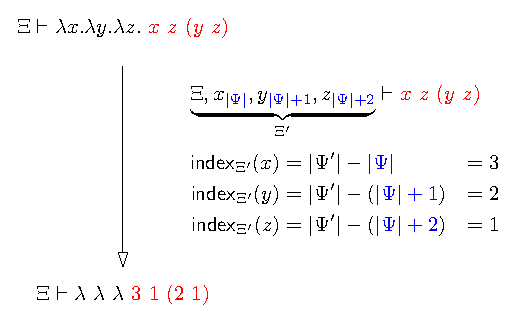
\includegraphics{figures/lf-indexing.eps}
\caption[Example of de Bruijn indices computation with respect to a lookup table]{%
Computation of de Bruijn indices for the $\mathbf{S}$-combinator using indexing context sizes stored in the lookup table.
The ambient \LF context $\Psi$ may be non-empty, in which case its bindings are included in the referencing environment $\Xi$.
This ensures that the combinator may be indexed correctly when it is nested under additional abstractions like in $\lambda w. (\lambda x. \lambda y. \lambda z.\ x\ z\ (y\ z))$.
The expression $x\ z\ (y\ z)$ is indexed with respect to $\Psi'$ since it is an \LF expression, and $\Psi'$ has $|\Psi| + 3$ entries since $x$, $y$ and $z$ are introduced by \LF~abstractions.
Variables in the referencing environment $\Xi'$ are annotated with the size of the \LF indexing context before each of them was added, namely $|\Psi|$ for $x$, $|\Psi| + 1$ for $y$ and $|\Psi| + 2$ for $z$.
}
\label{figure:lf-indexing}
\end{figure}

%Using the definition for referencing environments in \Beluga, the indexing phase is defined inductively as a set of translations functions.
%These are of the form $\Xi \vdash e \Translates_{s} e' \dashv \Xi'$, with $\Xi$ and $\Xi'$ being the input and output referencing environments respectively, and $e$ and $e'$ being the input and output term.
%This captures the notion that as a term is being indexed, data can be read from and written to the referencing environment.
%The translation $\Translates_{s}$ is split following the semantic classes of figure~\ref{figure:internal-syntax}, with $s$ being one of $K, A, M, U, C, \kappa, \tau, e$ and $i$, with the addition of $Mp, Cp$ and $p$ for \LF patterns, meta-object patterns and computation-level patterns respectively.


%A lookup for the definition bound to a fully qualified identifier in a referencing environment searches for the topmost frame whose tree of bindings contains the leading identifier in the fully qualified identifier.
%Once that frame is found, then its tree of bindings is traversed following the rest of the list of identifiers that forms the fully qualified identifier.
%The topmost entry in the stack associated with the trailing identifier is the one that's returned.
%If the traversal of the stack of frames fails or if no node in the tree of bindings can be found to match the fully qualified identifier, then the lookup fails.
%The stack structures at the level of frames and entries allow for identifier shadowing.
%On the other hand, the dictionaries speed up identifier lookups.

\subsection{Indexing \acs{LF} Kinds, Types and Terms}

Using the definition for referencing environments in \Beluga, the indexing phase is defined inductively as a family of translations functions indexed by the input's syntactic class.
These are of the form $\Xi \vdash \Indexes{e}{s}{\tilde e}$, with $e$ and $\tilde e$ being the input and output terms respectively, and $\Xi$ being the referencing environment.
However, that style of specification implicitly assumes that $\Xi$ is implemented as an immutable data structure.
To rectify this, a Hoare-style specification like $\Hoare{\Env = \Xi}{\Indexes{e}{s}{\tilde e}}{\Env = \Xi'}$ can be used instead, with $\Xi$ and $\Xi'$ being the initial and final states of the referencing environment.
The translation $\Indexes{}{s}{}$ is split following the semantic classes of figure~\ref{figure:internal-syntax}, with $s$ being one of $K, A, M, U, C, \kappa, \tau, e$ and $i$, with the addition of $Mp, Cp$ and $p$ for \LF patterns, meta-object patterns and computation-level patterns respectively.
This subsection focusses on indexing for \LF kinds, types and terms, and presents both styles of specifications $\Xi \vdash \Indexes{e}{s}{\tilde e}$ and $\Hoare{\Env = \Xi}{\Indexes{e}{s}{\tilde e}}{\Env = \Xi'}$, then demonstrates their equivalence.

First, the definitions for plain \LF kinds, types and terms are recalled below, with $a$ and $c$ standing for type-level and term-level constants respectively, and $x$ ranging over variables.

\begin{figure}[H]
\centering
\begin{tabular}{p{5.3cm} >{\raggedleft}p{1cm} r l}
Plain \LF kinds & $K$ & $\Coloneqq$ & $A \to K \mid \Pi x{:}A. K \mid \KWType$\\
Plain \LF types & $A, B$ & $\Coloneqq$ & $A\to B \mid \Pi x{:}A. B \mid a \mid A\ M_1\ M_2 \dots M_n$\\
Plain \LF terms & $M, N$ & $\Coloneqq$ & $x \mid c \mid \lambda x. M \mid M\ N_1\ N_2 \dots N_n \mid M : A$
\end{tabular}
\end{figure}

Then, the nameless counterparts of these \LF kinds, types and terms are defined, with $\tilde a$ and $\tilde c$ denoting the symbolic identifier corresponding to the type and term constants $a$ and $c$ respectively, and $\iota$ ranging over de Bruijn indices corresponding to variables.

\begin{figure}[H]
\centering
\begin{tabular}{p{5.3cm} >{\raggedleft}p{1cm} r l}
Nameless \LF kinds & $\tilde K$ & $\Coloneqq$ & $\tilde A \to \tilde K \mid \Pi_{\tilde A}\ \tilde K \mid \KWType$\\
Nameless \LF types & $\tilde A, \tilde B$ & $\Coloneqq$ & $\tilde A\to \tilde B \mid \Pi_{\tilde A}\ \tilde B \mid \tilde a \mid \tilde A\ \tilde M_1\ \tilde M_2 \dots \tilde M_n$\\
Nameless \LF terms & $\tilde M, \tilde N$ & $\Coloneqq$ & $\iota \mid \tilde c \mid \lambda\ \tilde M \mid \tilde M\ \tilde N_1\ \tilde N_2 \dots \tilde N_n \mid \tilde M : \tilde A$
\end{tabular}
\end{figure}

Indexing is first defined with respect to an immutable representation of the referencing environment $\Xi$ as an association list.
This algorithm is easy to implement, but comes at the expense of degraded runtime performance for lookups.
It is assumed that these computations take place in either a plain or module frame.

{\footnotesize
\begin{mdframed}[frametitle={$\boxed{\Xi \vdash \IndexesKind{K}{\tilde K}}$ : in the referencing environment $\Xi$, the \LF kind $K$ is indexed as $\tilde K$}]
\begin{equation}
\infer{
	\Xi \vdash \IndexesKind{A \to K}{\tilde A \to \tilde K}
}{
	\Xi \vdash \IndexesType{A}{\tilde A}
	& \Xi, \_ : \LFTerm \vdash \IndexesKind{K}{\tilde K}
}
\end{equation}

\begin{equation}
\infer{
	\Xi \vdash \IndexesKind{\Pi x{:}A. K}{\Pi_{\tilde A}\ \tilde K}
}{
	\Xi \vdash \IndexesType{A}{\tilde A}
	& \Xi, x : \LFTerm \vdash \IndexesKind{K}{\tilde K}
}
\end{equation}

\begin{equation}
\infer{
	\Xi \vdash \IndexesKind{\KWType}{\KWType}
}{}
\end{equation}
\end{mdframed}

\begin{mdframed}[frametitle={$\boxed{\Xi \vdash \IndexesType{A}{\tilde A}}$ : in the referencing environment $\Xi$, the \LF type $A$ is indexed as $\tilde A$}]
\begin{equation}
\infer{
	\Xi \vdash \IndexesType{A \to B}{\tilde A \to \tilde B}
}{
	\Xi \vdash \IndexesType{A}{\tilde A}
	& \Xi, \_ : \LFTerm \vdash \IndexesType{B}{\tilde B}
}
\end{equation}

\begin{equation}
\infer{
	\Xi \vdash \IndexesType{\Pi x{:}A. B}{\Pi_{\tilde A}\ \tilde B}
}{
	\Xi \vdash \IndexesType{A}{\tilde A}
	& \Xi, x : \LFTerm \vdash \IndexesType{B}{\tilde B}
}
\end{equation}

\begin{equation}
\infer{
	\Xi \vdash \IndexesType{a}{\tilde a}
}{
	\Lookup{a}{\Xi} = \tilde a : \LFTypeConst
}
\end{equation}

\begin{equation}
\infer{
	\Xi \vdash \IndexesType{A\ M_1\ M_2 \dots M_n}{\tilde A\ \tilde M_1\ \tilde M_2 \dots \tilde M_n}
}{
	\Xi \vdash \IndexesType{A}{\tilde A}
	& \left(\Xi \vdash \IndexesTerm{M_k}{\tilde M_k}\right)_{k \in \set{1, 2, \dots, n}}
}
\end{equation}
\end{mdframed}

\begin{mdframed}[frametitle={$\boxed{\Xi \vdash \IndexesTerm{M}{\tilde M}}$ : in the referencing environment $\Xi$, the \LF term $M$ is indexed as $\tilde M$}]
\begin{equation}
\infer{
	\Xi \vdash \IndexesTerm{x}{\iota}
}{
	\Lookup{x}{\Xi} = x : \LFTerm
	& \Index{\Psi}{x}{\Xi} = \iota
}
\end{equation}

\begin{equation}
\infer{
	\Xi \vdash \IndexesTerm{c}{\tilde c}
}{
	\Lookup{c}{\Xi} = \tilde c : \LFTermConst
}
\end{equation}

\begin{equation}
\infer{
	\Xi \vdash \IndexesTerm{\lambda x. M}{\lambda\ \tilde M}
}{
	\Xi, x : \LFTerm \vdash \IndexesTerm{M}{\tilde M}
}
\end{equation}

\begin{equation}
\infer{
	\Xi \vdash \IndexesType{M\ N_1\ N_2 \dots N_n}{\tilde M\ \tilde N_1\ \tilde N_2 \dots \tilde N_n}
}{
	\Xi \vdash \IndexesTerm{M}{\tilde M}
	& \left(\Xi \vdash \IndexesTerm{N_k}{\tilde N_k}\right)_{k \in \set{1, 2, \dots, n}}
}
\end{equation}

\begin{equation}
\infer{
	\Xi \vdash \IndexesType{M : A}{\tilde M : \tilde A}
}{
	\Xi \vdash \IndexesTerm{M}{\tilde M}
	& \Xi \vdash \IndexesType{A}{\tilde A}
}
\end{equation}
\end{mdframed}
}

In the implementation, indexing is imperative and defined with respect to a mutable referencing environment that is passed along for each computation.
The fact that computations may mutate the state is reflected formally using a Hoare-style specification.

{\footnotesize
\begin{mdframed}[frametitle={$\boxed{\Hoare{P}{\IndexesKind{K}{\tilde K}}{Q}}$ : the \LF kind $K$ is indexed as $\tilde K$ with precondition $P$ and postcondition $Q$}]
\begin{equation}
\infer{
	\Hoare{\Env = \Xi}{\IndexesKind{A \to K}{\tilde A \to \tilde K}}{\Env = \Unshift{\Psi}{\Xi''}}
}{
	\Hoare{\Env = \Xi}{\IndexesType{A}{\tilde A}}{\Env = \Xi'}
	& \Hoare{\Env = \Shift{\Psi}{\Xi'}}{\IndexesKind{K}{\tilde K}}{\Env = \Xi''}
}
\end{equation}

\begin{equation}
\infer{
	\Hoare{\Env = \Xi}{\IndexesKind{\Pi x{:}A. K}{\Pi_{\tilde A} \tilde K}}{\Env = \Pop{\Psi}{x}{\Xi''}}
}{
	\Hoare{\Env = \Xi}{\IndexesType{A}{\tilde A}}{\Env = \Xi'}
	& \Hoare{\Env = \Push{\Psi}{x : \LFTerm}{\Xi'}}{\IndexesKind{K}{\tilde K}}{\Env = \Xi''}
}
\end{equation}

\begin{equation}
\infer{
	\Hoare{\Env = \Xi}{\IndexesKind{\KWType}{\KWType}}{\Env = \Xi}
}{}
\end{equation}
\end{mdframed}

\begin{mdframed}[frametitle={$\boxed{\Hoare{P}{\IndexesType{A}{\tilde A}}{Q}}$ : the \LF type $A$ is indexed as $\tilde A$ with precondition $P$ and postcondition $Q$}]
\begin{equation}
\infer{
	\Hoare{\Env = \Xi}{\IndexesType{A \to B}{\tilde A \to \tilde B}}{\Env = \Unshift{\Psi}{\Xi''}}
}{
	\Hoare{\Env = \Xi}{\IndexesType{A}{\tilde A}}{\Env = \Xi'}
	& \Hoare{\Env = \Shift{\Psi}{\Xi'}}{\IndexesType{B}{\tilde B}}{\Env = \Xi''}
}
\end{equation}

\begin{equation}
\infer{
	\Hoare{\Env = \Xi}{\IndexesType{\Pi x{:}A. B}{\Pi_{\tilde A}\ \tilde B}}{\Env = \Pop{\Psi}{x}{\Xi''}}
}{
	\Hoare{\Env = \Xi}{\IndexesType{A}{\tilde A}}{\Env = \Xi'}
	& \Hoare{\Env = \Push{\Psi}{x : \LFTerm}{\Xi'}}{\IndexesType{B}{\tilde B}}{\Env = \Xi''}
}
\end{equation}

\begin{equation}
\infer{
	\Hoare{\Env = \Xi}{\IndexesType{a}{\tilde a}}{\Env = \Xi}
}{
	\Lookup{a}{\Xi} = \tilde a : \LFTypeConst
}
\end{equation}

\begin{equation}
\infer{
	\Hoare{\Env = \Xi}{\IndexesType{A\ M_1\ M_2 \dots M_n}{\tilde A\ \tilde M_1\ \tilde M_2 \dots \tilde M_n}}{\Env = \Xi_n}
}{
	\Hoare{\Env = \Xi}{\IndexesType{A}{\tilde A}}{\Env = \Xi_0}
	& \left(\Hoare{\Env = \Xi_{k - 1}}{\IndexesTerm{M_k}{\tilde M_k}}{\Env = \Xi_k}\right)_{k \in \set{1, 2, \dots, n}}
}
\end{equation}
\end{mdframed}

\begin{mdframed}[frametitle={$\boxed{\Hoare{P}{\IndexesTerm{M}{\tilde M}}{Q}}$ : the \LF term $M$ is indexed as $\tilde M$ with precondition $P$ and postcondition $Q$}]
\begin{equation}
\infer{
	\Hoare{\Env = \Xi}{\IndexesTerm{x}{\iota}}{\Env = \Xi}
}{
	\Lookup{x}{\Xi} = x : \LFTerm
	& \Index{\Psi}{x}{\Xi} = \iota
}
\end{equation}

\begin{equation}
\infer{
	\Hoare{\Env = \Xi}{\IndexesTerm{c}{\tilde c}}{\Env = \Xi}
}{
	\Lookup{c}{\Xi} = \tilde c : \LFTermConst
}
\end{equation}

\begin{equation}
\infer{
	\Hoare{\Env = \Xi}{\IndexesTerm{\lambda x. M}{\lambda\ \tilde M}}{\Env = \Pop{\Psi}{x}{\Xi'}}
}{
	\Hoare{\Env = \Push{\Psi}{x : \LFTerm}{\Xi}}{\IndexesTerm{M}{\tilde M}}{\Env = \Xi'}
}
\end{equation}

\begin{equation}
\infer{
	\Hoare{\Env = \Xi}{\IndexesTerm{M\ N_1\ N_2 \dots N_n}{\tilde M\ \tilde N_1\ \tilde N_2 \dots \tilde N_n}}{\Env = \Xi_n}
}{
	\Hoare{\Env = \Xi}{\IndexesTerm{M}{\tilde M}}{\Env = \Xi_0}
	& \left(\Hoare{\Env = \Xi_{k - 1}}{\IndexesTerm{N_k}{\tilde N_k}}{\Env = \Xi_k}\right)_{k \in \set{1, 2, \dots, n}}
}
\end{equation}

\begin{equation}
\infer{
	\Hoare{\Env = \Xi}{\IndexesTerm{M : A}{\tilde M : \tilde A}}{\Env = \Xi''}
}{
	\Hoare{\Env = \Xi}{\IndexesTerm{M}{\tilde M}}{\Env = \Xi'}
	& \Hoare{\Env = \Xi'}{\IndexesType{A}{\tilde A}}{\Env = \Xi''}
}
\end{equation}
\end{mdframed}
}

Neither formulation of the indexing algorithm is total since the identifier and index lookup operations fail for unbound identifiers.
In the immutable setting, recovering from such failures is trivial since no effects are applied to the association list of bindings.
On the other hand, the mutable setting does not make any guarantee as to the state of the referencing environment after a computation.
This potentially allows insertions to occur in an unpredictable order, and for deletions to unintentionally remove bindings that appear in outer frames of the initial referencing environment.
This next theorem certifies that that is not the case: if a binding removal occurs during indexing, then it is immediately preceded by the addition of that same binding.

In fact, the referencing environment is restored to its initial state after successfully indexing an \LF object.
This means that in the event of a failure during indexing, the environment has at least the bindings of its initial state.
Hence, pushing a new frame onto the referencing environment and popping it in case of failure is a sufficient mechanism to undo any and all effects on the state, which is paramount for incremental developments.
Additionally, since the ordering of add and remove operations is preserved, it follows that the computation of de Bruijn indices in the mutable setting are correct.

\begin{restatable}[Equivalence]{theorem}{equivalencetheorem}\label{theorem:equivalence}
The formalisms for indexing with respect to the immutable and mutable representations of the referencing environment are equivalent.
\begin{enumerate}
\item $\Hoare{\Env = \Xi}{\IndexesKind{K}{\tilde K}}{\Env = \Xi'}$ if and only if $\Xi \vdash \IndexesKind{K}{\tilde K}$ and $\Xi' = \Xi$.
\item $\Hoare{\Env = \Xi}{\IndexesType{A}{\tilde A}}{\Env = \Xi'}$ if and only if $\Xi \vdash \IndexesType{A}{\tilde A}$ and $\Xi' = \Xi$.
\item $\Hoare{\Env = \Xi}{\IndexesTerm{M}{\tilde M}}{\Env = \Xi'}$ if and only if $\Xi \vdash \IndexesTerm{M}{\tilde M}$ and $\Xi' = \Xi$.
\end{enumerate}
\end{restatable}

\begin{proof}
See appendix~\ref{chapter:indexing}.
\end{proof}

\begin{corollary}
Successfully indexing an \LF kind, type or term using the Hoare-style algorithm specification restores the referencing environment to its initial state.
\begin{enumerate}
\item If $\Hoare{\Env = \Xi}{\IndexesKind{K}{\tilde K}}{\Env = \Xi'}$, then $\Xi' = \Xi$.
\item If $\Hoare{\Env = \Xi}{\IndexesType{A}{\tilde A}}{\Env = \Xi'}$, then $\Xi' = \Xi$.
\item If $\Hoare{\Env = \Xi}{\IndexesTerm{M}{\tilde M}}{\Env = \Xi'}$, then $\Xi' = \Xi$.
\end{enumerate}
\end{corollary}

\section{Discussion}

As part of the reimplementation of the indexing phase, the referencing environment was first designed using immutable data structures.
Specifically, \acp{HAMT} were leveraged for the dictionaries mapping identifiers to stacks of bindings.
The indexing functions were then implemented using the state monad so that derived states could be passed on to later operations.
Having copies of the referencing environment for free during indexing would have facilitated incremental development because they could be attached to proof declarations to allow state rollbacks like in \Isabelle/\Isar with its context graphs.
In turn, checking out an incomplete theorem in \Harpoon would simply result in the referencing environment's copy being used for elaborating commands.
Unfortunately, the increased number of memory allocations, the overhead of insertions and removals in \acp{HAMT} and the lack of contiguity in the memory layout for the referencing environment incurred a decrease in runtime performance by a factor of roughly 10 for \Beluga's test suite.
This meant that running the indexing phase on a signature would take more time than type-checking it.
Thankfully, the indexing phase's implementation was loosely coupled with the representation of the referencing environment, and the state monad was used throughout.
This made it easy to substitute a mutable data structure for the referencing environment and recover runtime performance comparable to that of the legacy implementation of \Beluga.
Consequently, checking out incomplete proofs in \Harpoon now involves reconstructing the referencing environment using the internal \ac{AST}'s representation of the signature.

From a programming language implementation standpoint, the revised indexing phase simplifies the system's flow of information by decoupling it from the signature reconstruction store.
This opens up multiple opportunities, including proper unit-testing of the referencing environment structure and indexing functions.
Additionally, given \Beluga's design for signature-level declaration of constants, the indexing phase can be parallelized.
This is because the body of a signature-level declaration is guaranteed not to export non-constant identifiers.
This means that the referencing environment right before a signature-level can be constructed while disregarding most of the \ac{AST}.
As such, the declarations in a signature can first be traversed to preallocate symbolic identifiers for toplevel constants and store them in a queue.
Concurrent threads can then be assigned non-overlapping ranges of declarations to process, and the initial referencing environment for each can be constructed using only that queue.
Should this isolation for signature-level declarations be extended to the later phases of processing, concurrently type-checking programs could improve \Beluga's performance in large mechanizations.
